\documentclass[10pt,a4paper,final]{report}
\usepackage[utf8]{inputenc}
\usepackage{amsmath}
\usepackage{amsfonts}
\usepackage{amssymb}
\usepackage{graphicx}
\usepackage[ruled,vlined]{algorithm2e}
%\usepackage{multicols}

\author{Nisha Chandramoorthy}
\title{The Norbury Problem}

\begin{document}
\begin{titlepage}
\maketitle
\end{titlepage}

\section{Introduction}

Vortex Rings are volumes of non-zero vorticity in a fluid where the flow is predominantly poloidal. That is, in a Vortex Ring, the fluid assumes the shape of a torus and flows around the meridional cross section of the torus. Norbury's paper$\cite{norbury}$ describes a family of steady, axisymmetric Vortex Rings in an incompressible, inviscid fluid.

Rings in such a family can be described by a parameter $\alpha$ which varies between $\sqrt{2}$ for Hill's spherical vortex and $\approx 0$ for rings with very small cross section. These rings move in the surrounding fluid, which is at rest at infinity, without changing their shape, at a nearly constant translational speed normal to the plane of the circular axis of the torus. A numerical description of the shape of their meridional cross section has been dealt with in the paper$\cite{norbury}$. This report is concerned with achieving the same end by reworking the numerical method given in the paper.    
\\
\\
\begin{figure}


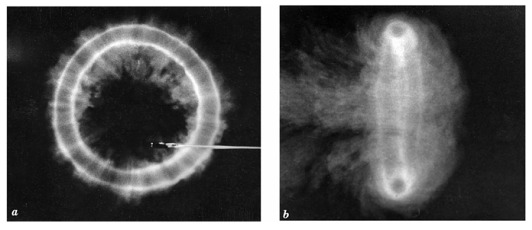
\includegraphics[scale=0.4]{rings.jpg}
\caption{vortex rings -front and side views.}

\end{figure}


\section{Formulation of the Problem(From the Paper$\cite{norbury}$)}
\subsection{Stream Function-Vorticity equation}
In a steady, incompressible, inviscid flow, the continuity equation is expressed as :
\begin{equation}
	\nabla . {\bf v} = 0
\end{equation}
So, a vector potential $(0, \Psi/r, 0)$ exists such that,
\begin{equation}
	{\bf v} = \nabla\times(0, \Psi/r,0) = (-\frac{1}{r}\frac{\partial\Psi}{\partial z}, 0, \frac{1}{r}\frac{\partial\Psi}{\partial r}),
\end{equation}
\\
where $\Psi(r,z) \equiv $ Stream Function in cylindrical coordinates.
\\
The Vorticity equation in this case is:
\\
\begin{equation}
	{\bf v}.\nabla(\omega/r) = 0
\end{equation}
This equation is trivially satisfied by the distribution of vorticity, 
\begin{equation}
	\omega = \Omega r \;\; \Omega = \;\; \text{constant}
\end{equation}
\\
The Stream Function $\Psi$ satisfies the following equation: 

\begin{equation}
 \left\lbrace\frac{\partial^2}{\partial r^2} -	
 \frac{1}{r}\frac{\partial}{\partial r} +
 \frac{\partial^2}{\partial z^2}\right\rbrace \Psi(r,z) =
	\nabla \times {\bf v} =
 \left\{\begin{aligned} 
        -\Omega r^2 \; &\text{inside}\; \partial \emph{A},\\
        0 \; &\text{outside} \; \partial A
       \end{aligned}
 \right\}
\end{equation}
\\
\begin{equation}
\begin{aligned}
	\Psi = k \; &\text{on} \, \partial A, \\
	\Psi + \frac{1}{2} W r^2 \rightarrow 0 \, &\text{as} \, r^2 + z^2 \rightarrow \infty
\end{aligned}
\end{equation}
\\
$k \equiv $ constant \\
$W \equiv $ Free Stream Velocity

\begin{figure}

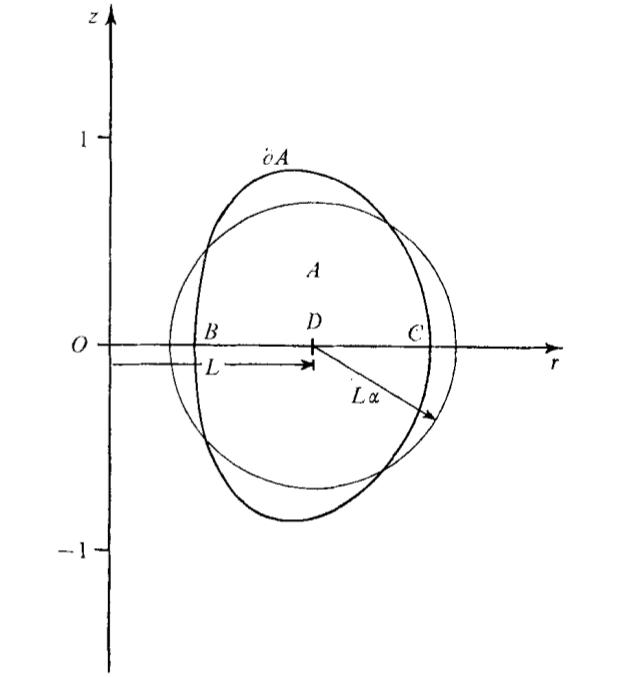
\includegraphics[scale=0.5]{shape.jpg}
\caption{Cross section A and boundary $\partial A$ shown in cylindrical coordinates. $\alpha$ is such that area of A = $\pi L^2 \alpha^2$}

\end{figure}

The solution , $\Psi$ , based on the fundamental solution of the Poisson equation is given by:
\\
\begin{equation}
	\Psi(r, z) = -\frac{1}{2}Wr^2 + 
	\frac{\Omega}{2\pi}\int \int_A \, 
	G(r, \hat{r}, z - \hat{z}) d\hat{r}d\hat{z}
\end{equation}
\\
where
\\
\begin{equation}
G(r, \hat{r}, z - \hat{z}) = \frac{1}{2} r \hat{r}^2 
\int_{-\pi}^{\pi} \frac{cos\, \hat{\lambda} d\hat{\lambda}}
{\lbrace r^2 + \hat{r}^2 - 2r\hat{r}cos\,\hat{\lambda} 
+ (z-\hat{z})^2 \rbrace^{\frac{1}{2}}}
\end{equation}
$G$ can be thought of as the stream function at $(r,z)$ of a singular vortex circle at $(\hat{r},\hat{z})$ having vorticity of delta-function type with circulation $2\pi\hat{r}$.
The problem thus reduces to solving for $\partial \emph{A}$ .
\\
\subsection{Non-linear Integral Equation}
The parameter $\alpha$ is introduced such that,
\begin{equation}
\text{area of }\;\emph{A}= \pi L^2 \alpha^2
\end{equation}

A change of Co-ordinates is employed from \emph{(r,z)} to \emph{(s,t)} using, 
\begin{align*}
	r &= 1 + s\; cos\,t  \\
	z &= sin\,t,
\end{align*}

Thus, if the symmetric curves $\partial \emph{A} (\alpha) $ are written as a fourier series,
\[
	s = f(t,\alpha) = \sum_{n=0}^{\infty} a_n(\alpha) cos \, nt
\]
%\\
where, $a_0$ and $a_1$ are determined from \\
1. area of $\emph{A} = \pi \alpha^2$ (After non-dimensionalization) \\
2. $s(0,\alpha) = s(\pi, \alpha)$, \\
%
We have the following non-linear integral equation that describes the boundary in terms of s and t:
\begin{equation}
k(\alpha) = -\frac{1}{2} W(\alpha)\{1 + f cos\;t\}^2 + 
\frac{1}{2\pi\alpha^2} \int_0^{2\pi} d\hat{t} \int_0^{\hat{f}}
 G(1 + f cos\;t,\; 1 + \hat{s}cos \:\hat{t}, \; f sin\: t - 
 \hat{s} sin\: \hat{t}) \; \hat{s} \; d\hat{s}  \;\;\;\;\;\; 0 \leq t \leq \pi   
\end{equation}
% 
Here, \emph{k} and \emph{W} have been non-dimensionalized.
%
\subsection{Introducing $P_\alpha$}
%
The vector {\bf X} is used to represent \emph{k}, \emph{W} and the set of unknown fourier coefficients that describe the boundary \emph{s(t)}. 
\\
$ {\bf X} \equiv (X_1, X_2, X_3, X_4, X_5,...) \equiv ({k},{W},{a_2}, {a_3}, {a_4}, ...)$
\\
%
A function $P_\alpha(t) $ is finally introduced to describe the integral equation. 
%
\begin{equation}
P_\alpha({\bf X}) (t) \equiv - X_1 - \frac{1}{2} X_2 (1 + {f} cos\, t)^2 + \frac{1}{2\pi\alpha^2} \int_0^{2\pi} 
d\hat{t} \times \int_0^{{\hat{f}}} G(1+ {f} cos\, t, 1 + \hat{s} cos \hat{t}, {f} \,sin \, t - \hat{s}\, 
sin\,\hat{t}) \hat{s} \, d\hat{s}  \;\;\;  (0\leq t \leq\pi)
\end{equation}
Assuming the function $P_\alpha$ is differentiable with respect to ${\bf X}$, Newton's Method is used to find the unknowns in ${\bf X}$.
\begin{align}
	\sum_{j=1}^N \frac{\partial P_\alpha}{\partial X_j} ({\bf X}^1) \times \delta_j &= -P_\alpha({\bf {X}}^{n-1}) & t = t_i \in [0, \pi] \;\; (i = 1, ..., N), \\
	{\bf {X}}^n &= {\bf {X}}^{n-1} + {\delta} & (n\geq 2).
\end{align}

Here, the number of fourier coefficients is reduced to N in order to obtain a discretized system of equations. The paper\cite{norbury} mentions that assuming $a_n = 0 , n \geq N$ does not affect the accuracy of the calculated boundary. 
%
So, we obtain a linear system of equations, 
\begin{equation}
	{\cal P} {\bf \delta} = {\cal B}
\end{equation}
%
where, in the nth iteration,\\
\\
\[
{\cal P}_{(i,j)} = \frac{\partial P_\alpha({\bf X^{n-1}},t_i)}{\partial X_j^{n-1}}
\] and \\
\[
{\cal B}_{i} = - P_\alpha({\bf X^{n-1}},t_i)
\]
But, in the paper and in this report, the initial seed for ${\bf X}$ and hence,
the subsequent vectors, are within 0.01 of the actual value. In that case, retaining the left hand side of the system of equations, ie, ${\cal P}$ as it was in the first iteration, across iterations, doesn't affect the accuracy much. Therefore, 
\\
\\
\[
{\cal P} \equiv  
\begin{bmatrix}
\partial P_\alpha^{t_1}/\partial X_1^1 & \partial P_\alpha^{t_1}/\partial X_2^1 & . & . & \partial P_\alpha^{t_1}/\partial X_N^1 \\ 
. & . & . & . & . \\ 
. & . & \partial P_\alpha^{t_i}/\partial X_j^1 & . & . \\ 
. & . & . & . & . \\ 
\partial P_\alpha^{t_N}/\partial X_1^1 & . & . & . & \partial P_\alpha^{t_N}/\partial X_N^1
\end{bmatrix} 
\]
where 
\[
P_\alpha^{t_i} \equiv P_\alpha(\bf{X^1},t_i).
\] 
%
\\
and,
\[
\bf \delta \equiv
\begin{bmatrix}
\delta_1 \\
. \\
. \\
\delta_N
\end{bmatrix}
\]

and
\[
{\cal B} \equiv 
\begin{bmatrix}		
-P_\alpha^{t_1}({\bf X^{n-1}}) \\ 
. \\ 
. \\ 
-P_\alpha^{t_N}({\bf X^{n-1}})
\end{bmatrix} 
\].

\section{Solution}
\subsection{Constructing ${\cal P}$}
%
In the program, the table given in the paper\cite{norbury} was used to provide the initial value of {\bf X}.
Each term in ${\cal P}$ is calculated as a simple forward difference with $\Delta = 0.008$. The value of $\Delta$ is not sacrosanct; However, the accuracy didn't improve on testing with lower values of $\Delta$. 
Now, evaluating $P$ given an $\bf X$ and $\alpha$ is all that remains. 
\begin{equation}
P_\alpha({\bf X})(t) = -X_1 - 1/2 X_2 (1 + fcos\: t)^2 + 
\frac{1}{2\pi\alpha^2} \int_0^{2\pi} \: d\hat{t} \times 
\int_0^{\hat{f}} \: G(1+fcos\: t,       
\; 1 + \hat{s}cos {\hat{t}} , f sin t - 
\hat{s}sin \hat{t}) \: \hat{s} \; \hat{ds}
%
\end{equation}

\subsection{Some Observations}
For the repeated integral in the above expression, three combinations of quadrature rules were tried out with the inner integral (whose integrand contains G) always being evaluated using Gauss Quadrature and the outer integral being evaluated using Gauss quadrature, Trapezoidal rule and Simpson's rule. 

 Using Gauss Quadrature for the inner integral successfully avoided the singularities in $(s,t)$, but an accuracy warning was flashed while running the program, now and then. The integrand, the inner integral, might be such that neglecting the singularities introduces irreconcilable inaccuracies, especially for higher values of $\alpha \geq 0.9$\cite{singularity}. 
\\
\\
\\
Using Gauss Quadrature for the inner integral and Simpson's Rule for the outer fails for high values of $\alpha$. Either singularities are encountered or the values of the fourier coefficients $a2...a17$ are skewed by inaccuracy to such an extent that $a0^2$ or $a1^2$ turns out to be negative. The only rationale behind using this combination of quadrature rules might be good concurrence of results with Gauss Quadrature for moderate values of $\alpha \; (0.4\leq\alpha\leq0.8) $ with a mere 100 points of $\hat{t}$ which takes very less time per iteration.   
The method used in the paper involves calculating the integral around the logarithmic singularity as well but locating the singularity might be difficult. 
\\
\\
\\
The table below shows the values of the fourier coefficients calculated after 10 iterations calculated starting with the approximations given in the paper and using Gauss quadrature for both integrals. The values in the paper\cite{norbury} indeed had upto 4 digits of accuracy, as mentioned.The values of $\delta$ after 10 iterations were close to machine zero. 
  
\subsection{Sample Revised Approximations(After 10 iterations)}
\begin{tabular}{|c|c|c|c|c|c|}
\hline
\rule[-1ex]{0pt}{2.5ex} $\alpha$ & 0.2 & 0.4 & 0.8 & 0.9 & 1.2 \\ 
\hline 
\rule[-1ex]{0pt}{2.5ex} k & 4.32315243e-01 & 2.08493879e-01 & 4.70191410e-02 & 3.01704096e-02 & 0.00444298 \\ 
\hline
\rule[-1ex]{0pt}{2.5ex} W & 8.50400253e-01 & 6.58798074e-01 & 4.42788476e-01 & 4.04304753e-01 & 0.31360119 \\ 
\hline
\rule[-1ex]{0pt}{2.5ex} $a_2$ & -6.80633236e-03 & -3.79506001e-02 &  -1.76143656e-01 & -2.20779958e-01  & -0.35422411 \\ 
\hline 
\rule[-1ex]{0pt}{2.5ex} $a_3$ & 5.44669076e-04 &  5.89099833e-03 & 5.03848570e-02 & 6.92465149e-02 & 0.1408757 \\ 
\hline 
\rule[-1ex]{0pt}{2.5ex} $a_4$ & 1.30508091e-04 & 1.84504211e-03  & 1.78505437e-02 &  2.46352966e-02  & 0.0429047 \\ 
\hline 
\rule[-1ex]{0pt}{2.5ex} $a_5$ & -3.29985426e-05 & -9.47887529e-04  & -1.83676605e-02 & -2.84204620e-02 &  -0.07226434 \\ 
\hline 
\rule[-1ex]{0pt}{2.5ex} $a_6$ & 2.05231221e-07  &  6.28026855e-05 &  3.45786437e-03 & 6.09303239e-03 &  0.02355147 \\ 
\hline 
\rule[-1ex]{0pt}{2.5ex} $a_7$ & 1.18245093e-06 &  8.43575167e-05  & 3.49305422e-03  & 6.09073634e-03 & 0.01837474 \\ 
\hline 
\rule[-1ex]{0pt}{2.5ex} $a_8$ & -8.70315887e-08  & -3.18950086e-05  & -2.72848015e-03 & -5.27364944e-03 & -0.02276031 \\ 
\hline 
\rule[-1ex]{0pt}{2.5ex} $a_9$ & -9.27144092e-09  &  -3.64817888e-07  & 2.72504999e-04 & 6.16848170e-04 & 0.00512039 \\ 
\hline 
\rule[-1ex]{0pt}{2.5ex} $a_{10}$ & -4.41786108e-09 & 4.11178618e-06 & 7.50104943e-04  & 1.65176386e-03 & 0.0087044 \\ 
\hline 
\rule[-1ex]{0pt}{2.5ex} $a_{11}$ & 2.19866428e-08 &  -1.19485707e-06  & -4.81736326e-04 & -1.15855392e-03 & -0.00857991 \\ 
\hline 
\rule[-1ex]{0pt}{2.5ex} $a_{12}$ & -3.04545907e-09 &  1.69784178e-07  & -3.46755236e-06 & -2.49383793e-07 &  0.00103893 \\ 
\hline 
\rule[-1ex]{0pt}{2.5ex} $a_{13}$ & 3.35073056e-05  &  -8.27994675e-08 &  1.70012669e-04  & 4.66940922e-04 & 0.00411869 \\ 
\hline 
\rule[-1ex]{0pt}{2.5ex} $a_{14}$ & -1.47724818e-07 & -8.84480805e-08 & -9.38656694e-05  & -2.81972375e-04 & -0.00373116 \\ 
\hline 
\rule[-1ex]{0pt}{2.5ex} $a_{15}$ & -1.65694037e-08 &  -2.06670426e-09 & -3.90227037e-06 & -4.55700833e-06 & 0.00066228 \\ 
\hline 
\rule[-1ex]{0pt}{2.5ex} $a_{16}$ &   4.77222260e-09 &  5.76831633e-08 & 3.50430194e-05   & 1.16375037e-04  &  0.00174839 \\ 
\hline 
\rule[-1ex]{0pt}{2.5ex} $a_{17}$ & -1.89693797e-08 &  -1.34775847e-08 & -1.72326454e-05  & -6.21983756e-05 &  -0.00125495\\ 
\hline 
\end{tabular} 
%
\subsection{Using Trapezoid Rule for the Outer Integral}
The advantages of using Trapezoid Rule over Gauss quadrature or Simpson's Rule, for the outer integral (in $\hat{t}$) are two fold. First, while Simpson's Rule failed for $\alpha \geq 1$ and for low values of $\alpha$, Trapezoid Rule works upto $\alpha=1.3$ and works well for low values of $\alpha$. For higher values of alpha (say, $\alpha = \sqrt{2}$), Gauss Quadrature is the only successful choice. The other advantage of using Trapezoid Rule is it seems to be accurate when verified against the paper within few iterations and even with a 100 points of the outer integral. The table below assists comparison between the Gauss Quadrature solution and the Trapezoid Rule solution for one value of $\alpha$. 
\\
\\
Accuracy warnings from the Gauss quadrature function used to evaluate the inner integral persisted with Trapezoid Rule as well. But, the difference reported by the function was lower ($<10^-7$) when the number of points of the outer integral was increased. (Table below shows the results for a 1000 points).  
\\
\\
On splitting the inner integral into smaller intervals and summing up the Gauss Quadrature result from each of the intervals resulted in NaNs often, for high values of alpha(See for example the commit mentioned\cite{commit}). In cases where NaNs don't occur, the results are still riddled with accuracy warnings.
%
%
\\
\\
\subsection{Revised Approximations using Trapezoid Rule}
\begin{tabular}{|c|c|c|c|c|c|}
\hline
\rule[-1ex]{0pt}{2.5ex} $\alpha$ & 0.2 & 0.8 & 0.8(Gauss) & 1.2(1000) \\ 
\hline 
\rule[-1ex]{0pt}{2.5ex} $k$ &  4.32334181e-01 & 4.70294764e-02 &  4.70191410e-02 & 4.43553708e-03 \\ 
\hline
\rule[-1ex]{0pt}{2.5ex} $W$ & 8.50411349e-01 & 4.42745289e-01  & 4.42788476e-01 & 3.13598460e-01 \\ 
\hline
\rule[-1ex]{0pt}{2.5ex} $a_0$ & 1.9994e-01 & 7.88827988e-01  & 0.78882493604551895 & 1.16585202e+00 \\ 
\hline
\rule[-1ex]{0pt}{2.5ex} $a_1$ & -5.7688e-04 & -3.57476386e-02  & -0.03544989714622 &  -8.70113455e-02 \\
\hline 
\rule[-1ex]{0pt}{2.5ex} $a_2$ & -6.7971e-03 & -1.75952543e-01   &  -1.76143656e-01 &  -3.54259796e-01  \\ 
\hline 
\rule[-1ex]{0pt}{2.5ex} $a_3$ & 6.0350e-04 &  5.06992932e-02   & 5.03848570e-02 & 1.40823346e-01 \\ 
\hline 
\rule[-1ex]{0pt}{2.5ex} $a_4$ & 1.3504e-04 &   1.78213320e-02  & 1.78505437e-02 &  4.29391074e-02\\ 
\hline 
\rule[-1ex]{0pt}{2.5ex} $a_5$ & -3.8278e-05 &  -1.84897416e-02 & -1.83676605e-02 & -7.22076492e-02 \\ 
\hline 
\rule[-1ex]{0pt}{2.5ex} $a_6$ &  1.1277e-05  &  3.49254209e-03  &  3.45786437e-03 & 2.34842673e-02 \\ 
\hline 
\rule[-1ex]{0pt}{2.5ex} $a_7$ & 3.2169e-06 & 3.57317767e-03   & 3.49305422e-03  & 1.83389043e-02  \\ 
\hline 
\rule[-1ex]{0pt}{2.5ex} $a_8$ & -3.1245e-07  & -2.78799713e-03   & -2.72848015e-03 &  -2.27561432e-02  \\ 
\hline 
\rule[-1ex]{0pt}{2.5ex} $a_9$ & 5.3231e-06 &  2.97416502e-04  & 2.72504999e-04 & 5.10783875e-03\\ 
\hline 
\rule[-1ex]{0pt}{2.5ex} $a_{10}$ & 1.2277e-06 & 7.77757697e-04  & 7.50104943e-04  & 8.70845393e-03  \\ 
\hline 
\rule[-1ex]{0pt}{2.5ex} $a_{11}$ & 1.9845e-08 & -5.01317300e-04 & -4.81736326e-04 & -8.57899098e-03 \\ 
\hline 
\rule[-1ex]{0pt}{2.5ex} $a_{12}$ & 2.9275e-06  &   6.01049171e-06    & -3.46755236e-06 & 1.03481374e-03 \\ 
\hline 
\rule[-1ex]{0pt}{2.5ex} $a_{13}$ & 1.0975e-06  &   1.85182586e-04 &  1.70012669e-04  & 4.12307998e-03\\ 
\hline 
\rule[-1ex]{0pt}{2.5ex} $a_{14}$ & 6.8963e-08  &  -1.03841883e-04   & -9.38656694e-05  & -3.72739280e-03   \\ 
\hline 
\rule[-1ex]{0pt}{2.5ex} $a_{15}$ & 1.8608e-06  &   4.60135141e-06 & -3.90227037e-06 & -6.58277134e-04\\ 
\hline 
\rule[-1ex]{0pt}{2.5ex} $a_{16}$ &  1.4492e-06  & 4.47152884e-05  & 3.50430194e-05   &  1.74696555e-03 \\ 
\hline 
\rule[-1ex]{0pt}{2.5ex} $a_{17}$ & 1.3571e-07 &  -2.09738425e-05 & -1.72326454e-05  & -1.25346043e-03 \\ 
\hline 
\end{tabular} 
		
\section{Algorithm}
\begin{algorithm}
\DontPrintSemicolon
\KwData{$\alpha$, ${\bf X^0} \equiv \{k,W,a_2,a_3...a_x\}$}
\KwResult{${\bf X^{m}}$ - Updated value of ${\bf X}$ after $m$ iterations}
$\Delta \longleftarrow 0.008$ \; 
$m \longleftarrow 9$ \;
$N \longleftarrow x+2$ \; 
\For{$i \longleftarrow 0$ \KwTo $N$}
{
	$P_1\longleftarrow P_\alpha({\bf X}, t_i)$ \;	
	\For{$j \longleftarrow 0$ \KwTo $N$}
	{
		$P_2 \longleftarrow P_\alpha({\bf X}(Where X_j \longleftarrow
		X_j + \Delta), t_i)$\; 
		${\cal P}(i,j) \longleftarrow (P_2 - P_1)/\Delta$\;
		}
	\nlset{UPDATE ${\cal B}$} ${\cal B}(i) \longleftarrow - P_1$ \; \label{upB} 

} 

\For{$n \longleftarrow 0$ \KwTo $m$}
{
	\tcc*{${\cal P}$ remains the same} \;
	$\delta \longleftarrow \text{solve}({\cal P},{\cal B})$ \;
	$X^{n+1} \longleftarrow X^{n} + \delta$ \;
	Update ${\cal B}$ as in \ref{upB}
}
\caption{Complete Numerical Procedure}
\end{algorithm}
\begin{algorithm}
\DontPrintSemicolon
\KwData{Current Value of {\bf X} , t}
\KwResult{$P_\alpha({\bf X},t)$}
$a_1 \longleftarrow -\{a_3 + a_5 + ...\}$ \;
$a_0 \longleftarrow \alpha^2 - \frac{1}{2}\{a_1^2 + a_2^2+...+ a_N^2\}$ \;
$f \longleftarrow f(t,\alpha) \longleftarrow \sum_{i=0}^N a_i cos\,i\,t$ \;
$t_1 \longleftarrow -k$ \;
$t_2 \longleftarrow -\frac{1}{2} W \times (1 + f cos \; t)^2$ \;
$t_3 \longleftarrow \frac{1}{2\pi\alpha^2} outerIntegral({\bf X}, t)$ \; \tcc*{Compute outer integral using Gauss Quadrature
or Simpson's Rule or Trapezoid Rule}
$P_\alpha \longleftarrow t_1 + t_2 + t_3$ \;
\caption{Method $P_\alpha({\bf X},t)$}
\end{algorithm}

\begin{algorithm}
\DontPrintSemicolon
\LinesNumbered
\KwData{Current Value of {\bf X},$a_0, a_1, \alpha$, t}
\KwResult{$\int_0^{2\pi} d\hat{t} \times \int_0^{\hat{f}} G(1 + f\, cos\, t, 1 + \hat{s} cos \, 
\hat{t}, f sin\, t - \hat{s} sin \hat{t} ) \, \hat{s} d\hat{s}$}
Divide interval $[0,2\pi]$ into L points \;
Use Trapezoid Rule for all $\alpha$ except at the extremes where Gauss Quadrature can be used. \;
\tcc*{To find the integrand of the outer integral} 
\Begin{
	$\hat{f} \longleftarrow f(\hat{t}, \alpha) \longleftarrow \sum_{i=0}^N
	 a_i \times cos \,i \hat{t} $ \;
	Compute $iint \longleftarrow innerIntegral(\hat{f})$\;	 
	\Begin{
		\tcc*{Inner Integral}
		Compute integral using Gauss Quadrature between the limits $0$ and $\hat{f}$. \;
		\tcc*{To find the Integrand of the inner integral}
		\Begin{
		$innerIntegrand \longleftarrow \hat{s} \times G(r\longleftarrow 1 + f\, cos\, t,
		\hat{r}\longleftarrow 1 + \hat{s} cos \, \hat{t}, z - \hat{z} \longleftarrow 
		f sin\, t - \hat{s} sin \hat{t})$ \;
		$\xi \longleftarrow \sqrt{\{ 4r\hat{r}/({(r + \hat{r})}^2 + {(z-\hat{z})}^2) \}}$ \;
		Compute $G(r,\hat{r},z-\hat{z}) \, \longleftarrow \hat{r}\{{(r+\hat{r})}^2 +
		{(z - \hat{z})}^2\}^\frac{1}{2} \{(1 - \frac{1}{2} \xi^2) EllipticK(\xi) - EllipticE(\xi)\}
		$ \;
		}
	} 
	  

}

\caption{Method $outerIntegral({\bf X},t)$}
\end{algorithm}



\begin{thebibliography}{9}

\bibitem{norbury}
 J. Norbury,
\emph{A Family of Steady Vortex Rings},\\
J. Fluid Mech. 1973

\bibitem{singularity}
 D. S. Lubinsky, P. Rabinowitz,
\emph{Rates of convergence of Gaussian quadrature for singular integrands} ,\\ 
J. Math. Comp. 43 (1984), 219-242 

\bibitem{commit}
Python Program implementing the procedure mentioned in this report.
\emph{https://github.com/nishaChandramoorthy/VortexMethods.git} \\
Commit SHA1: 4b672518, \\


\end{thebibliography}

\end{document}